
\chapter{Modèle de chargement}
\label{ch:loading-model}

Ce chapitre traite des mécanismes de chargement implémenté pour le système de
module.  Dans notre implémentation, les modules sont référés par un nom
symbolique plutôt que leur emplacement sur le système de fichier. Elle garantit
l'ordre dans lequel ils sont chargés et aussi le chargement unique de chaque
module. Pour permettre la diffusion des modules, nous avons ajouté un mécanisme
d'installation automatique et de chargement des modules à la volée.

Un système est composé d'un ensemble de modules qui interagissent entre eux.
L'interaction entre les modules est dans un contexte statique ou dynamique.
Dans le contexte statique, les modules sont incorporés au sein de
l'application, ils n'ont pas besoin d'être chargés. Dans le contexte dynamique,
les modules sont externes à l'application et requièrent un chargement
dynamique.  Le chargement dynamique de modules est une partie importante dans
un système de modules, il permet l'utilisation de modules externes.

La diffusion des modules requiert que le chargement de modules qui ne sont
pas encore installés soit effectué durant l'exécution.

\section{Chargement des bibliothèques}

%La collection des modules s'effectue au sein d'un

Le chargement d'une bibliothèque Scheme (ou module) dans Gambit est séparé en
plusieurs niveaux. Il y a la phase de recherche du module et de ses dépendances
qui valide la présence, sur le système de fichier ou en mémoire, de tous les
modules nécessaires.  Ensuite, le module et ses dépendances sont chargés dans un
ordre qui respecte les relations de dépendance.  Un module est soit sur le
système de fichier ou déjà en mémoire.  L'emplacement des bibliothèques sur le système de
fichier est lié par défaut aux chemins spécifiés par le
\lstinline{##module-search-order} qui a comme défaut \lstinline{~~lib} et
\lstinline{~~userlib}.

La procédure exacte de chargement des bibliothèques par \texttt{import} n'est pas
spécifiée par le standard R7RS. Le standard spécifie seulement une syntaxe de
base et le comportement principal qui est requis. L'importation d'une
bibliothèque doit charger la bibliothèque et rendre ses fonctionnalités
disponibles dans le contexte où l'importation a eu lieu (qui peut soit venir d'un
programme principal ou d'une bibliothèque).

Le chargement d'une bibliothèque peut-être effectuée à l'exécution par
l'utilisation de \texttt{eval} (par \texttt{load}) pour les fichiers source et
\texttt{load-object-file} pour les bibliothèques compilées. Cette recherche
peut aussi avoir lieu durant l'édition des liens en utilisant les méta-infos
contenues dans les fichiers \textbf{.c} qui sont chacun compilés par le compilateur C
en \textbf{.o} et lié par l'éditeur de lien.

\section{Modèle statique}

% XXX: Puisque toutes les dépendances sont dans l'application finale, il suffit de distribuer celui-ci/celle-ci.

Le modèle de bibliothèque statique consiste à intégrer la bibliothèque dans le
fichier exécutable de l'application finale. La bibliothèque n'a donc pas besoin
d'être chargée durant l'exécution. L'avantage du modèle statique est sur le
plan du déploiement.  Puisque toutes les dépendances sont dans l'application
finale, il suffit de distribuer celui-ci. Le compilateur Gambit supporte un
modèle statique pour des programmes simples. Compiler une application liée
statiquement est possible de façon manuelle. Pour lier statiquement deux
fichiers Scheme simples, il suffit d'invoquer le \texttt{gsc} comme suit:

\begin{center}
  \lstset{language={Scheme}}
\begin{mplisting}{0.4}
  $ gsc -exe file1.scm file2.scm
\end{mplisting}
\end{center}

% Par la contrainte des systèmes, le premier type de bibliothèques utilisé
% étaient dit statique.  Elles consistaient en un regroupement logique de
% plusieurs fichiers objets en un archive (.a). La création d'une bibliothèque
% statique peut s'effectuer avec l'utilitaire \verb|ar|. Lorsque que programme se
% lie à une bibliothèque statique, il inclut tout simplement l'ensemble des
% procédures contenu dans les fichiers objets. L'avantage des bibliothèques
% statiques est de regrouper plusieurs fonctionnalité commune en un seul concept,
% par exemple la bibliothèque mathématique \verb|libm.a| qui contient les
% fonctions mathématique (i.e. \verb|cos|, \verb|sin|).  En plus,  fait que le
% processus d'édition des liens, qui consiste à associer les noms des
% fonctionnalités avec leur valeur (AMBIGU), n'est effectué juste une fois. Une
% liaison avec une bibliothèque statique \verb|libfoo.a| qui contient le fichier
% objet \verb|foo.o| est équivalent à une liaison directe avec le fichier
% \verb|foo.o|.

% \begin{figure}[ht]
%     \begin{minipage}[t]{0.5\textwidth}
% \begin{verbatim}
% # Création de la bibliothèque statique libfoo.a
% ar rcs libfoo.a foo.o
% # Création de l'exécutable main.exe
% ld -o main.exe main.o libfoo.a
% \end{verbatim}
%     \end{minipage}
%     \caption{Exemple de création de bibliothèque statique suivit d'un exemple
%     d'utilisation.}
% \end{figure}


Un des problèmes du modèle statique est le coût lié à la maintenance.  Les
programmes qui utilisent des bibliothèques statiques ne permettent pas une
construction modulaire. La mise à niveau d'une des bibliothèques statiques
nécessite la recompilation du programme au complet. En plus, cela n'est pas
adapté pour des applications évolutives qui peuvent être étendues
par l'utilisateur. Une solution qui a été adoptée est le
modèle dynamique, présenté dans la prochaine section. Cela offre une plus grande
flexibilité dans le déploiement des programmes.


\section{Modèle dynamique}
\label{sec:ch4_model_dynamic}

%XXX: comprend pas?
Dans le modèle dynamique, chaque module externe est séparé durant l'exécution.
L'application contient les informations pour extraire les fonctionnalités des
modules durant l'exécution. Le déploiement d'une application nécessite la
distribution de toutes les dépendances directes et indirectes.  Les
bibliothèques partagées offrent plusieurs avantages par rapport aux
bibliothèques statiques.

Dans ce modèle les bibliothèques sont liées au programme durant l'exécution. Cela
nécessite que les bibliothèques soient organisées sur le système de fichier d'une façon
distinguable. Chaque module doit posséder un nom unique qui permet d'y référer.
Ce nom unique va être utilisé lors de la collection des dépendances.


%Les bibliothèques
%sont soit en code source ou compilé nativement avec l'extension (\textit{.oN})
%où le N correspond à la version du binaire qui commence à 1.


La recherche des bibliothèques est effectuée dans un ordre spécifique
indépendant de la spécification.  L'algorithme de recherche des bibliothèques
prend en paramètre le nom de la bibliothèque et retourne le chemin absolu
correspondant à son emplacement dans l'arborescence du système de fichier. Les
bibliothèques sont situées dans différents répertoires:
le répertoire des bibliothèques système (\lstinline{~~lib}) et le
répertoire des bibliothèques utilisateur (\lstinline{~~userlib}) ou des répertoires
explicitement ajoutés au <<module search order>>.

% \begin{itemize}
%   %% XXX: directory where the executable is located (usefull for devel no need to install the module). collecté
%   \item \verb|origin/dummy.sld|
%   \item \verb|origin/dummy/dummy.sld|
%   \item \verb|~~userlib/dummy.sld|
%   \item \verb|~~userlib/dummy/dummy.sld|
%   \item \verb|~~lib/dummy.sld|
%   \item \verb|~~lib/dummy/dummy.sld|
% \end{itemize}

Chaque module possède trois niveaux d'initialisation dans le système numérotés
de 0 à 2. Le niveau 0 indique que le module est collecté en mémoire, mais non
initialisé. Le niveau 1 indique que l'initialisation de bas-niveau a été
complétée et que le descripteur Scheme du module a été récupéré. Le niveau 2
marque les modules chargés dont toutes les définitions  et expressions au
niveau  principales (<<top level>>) ont été evaluées et donc le module est prêt
à être utilisé.  \\

% \begin{figure}[h]
%   \lstset{language={Scheme},frame=single}
%   \begin{mplisting}{1}
% > (##get-module '_zlib)
% #(_zlib
%   0
%   #(#(_zlib) #(_digest) () 1 #<procedure #2> #<foreign #3 0x7f0514907740>))
% \end{mplisting}
% \end{figure}
\begin{figure}[h]
  \lstset{language={Scheme},frame=single}
  \begin{mplisting}{1}
> (define mods (##collect-modules '(_zlib)))
> mods
(#(_digest 0 #(#(_digest) #() () 1 #<procedure #2> ...))
 #(_zlib 0 #(#(_zlib) #(_digest) () 1 #<procedure #4> ...)))
> (##init-modules mods)
#t
> ##registered-modules
(#(_digest 2 #(#(_digest) #() () 1 #<procedure #2 _digest#> ...))
 #(_zlib 2 #(#(_zlib) #(_digest) () 1 #<procedure #4 _zlib#> ...))
 ...)
\end{mplisting}
  \caption{Un exemple qui montre la collection des modules à partir du module
    \texttt{\_zlib} suivit de l'initialisation des modules collectés. La collection
    des modules est effectuée par la procédure \texttt{\#\#collect-modules}. L'ensemble
    des modules retournés sont initialisés par la procédure \texttt{\#\#init-modules}.
    Les enregistrements des modules \texttt{\_zlib} et \texttt{\_digest} ont été ajoutés
    à la liste des modules enregistrés (variable \texttt{\#\#registered-modules}).}
\end{figure}

\begin{figure}[ht]
  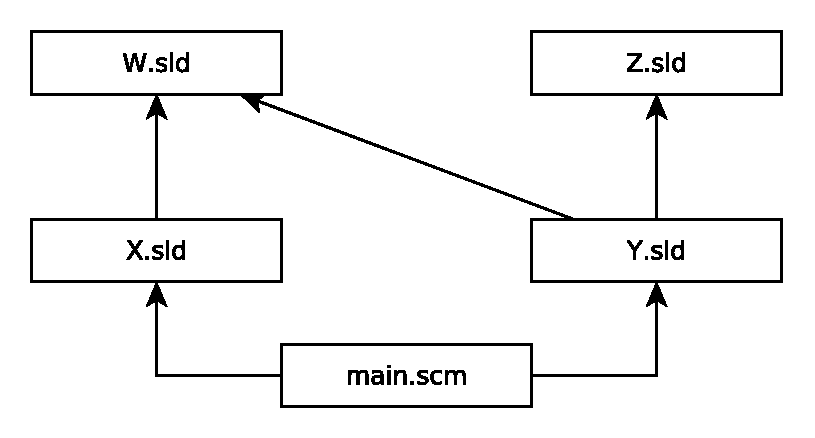
\includegraphics{figures/system-example}
  \caption{Un exemple d'un système fictif composé de différents modules.
  Le module principal se nomme \textbf{main.scm} avec l'extension \textbf{.scm}
  et les bibliothèques ont l'extension \textbf{.sld}}
  \label{fig:system-dependency-example}
\end{figure}


Dans l'exemple à la figure~\ref{fig:system-dependency-example}, l'exécution du module principal
\textbf{main.scm} déclenche la collection des modules X et Y, qui récursivement
déclenche la collection de W et Z.  L'algorithme de collection des modules gère
les modules qui apparaissent plusieurs fois au sein du graphe et les cycles.  Après la
collection de tous ces modules, le descripteur de module est
récupéré par un appel aux primitives du système d'exploitation si compilé.


\subsection{Module compilé dans Gambit}
% La construction d'un programme peut s'effectuer de façon modulaire; chaque
% composantes du programme peuvent être construites en séparément.  La
% modification d'une des bibliothèques partagés utilisés par
% le programme ne nécessite pas la recompilation de celui-ci. Le nom qui est
% donné à l'entité qui résout les noms des fonctionnalités est l'éditeur de liens (\textit{dynamic linker}).
% Habituellement les bibliothèques exportent des fonctions, mais il peuvent aussi
% exporter plusieurs types de données comme des entiers, des nombres à virgules,
% des chaînes de caractères et des données composites (structures). Chacune de ces données est
% associées à un nom unique (symbole) au sein de la bibliothèque.
% Il n'est pas possible d'avoir deux bibliothèques statiques qui exportent une
% fonctionnalité avec le même nom au sein d'une même application, alors qu'avec
% les bibliothèques partagés c'est possible. Cela limite le choix des
% bibliothèques qui peuvent être utilisé simultanément au sein du programme;
% chaque bibliothèque doit avoir un ensemble de nom de fonctionnalité distinct
% des autres. Puisque la résolution d'une fonctionnalité retourne la première
% occurrence trouvée, il n'y a rien qui empêche d'avoir plus d'une fonctionnalité
% associée au même nom.

Les modules dans Gambit peuvent être compilés pour plus de performance en
bibliothèque dynamique. Les programmes principaux peuvent être compilés en
exécutable.  Gambit permet l'utilisation de bibliothèques statiques et
dynamiques.\\

\begin{figure}[ht]
  \centering
  \lstset{language={Scheme},frame=single}

  \begin{mplisting}{0.5}
;; fib.scm
(define (fib n)
  (if (< n 2)
      n
      (+ (fib (- n 1))
         (fib (- n 2)))))
\end{mplisting}
  \caption{Un module qui implémente la fonction mathématique \texttt{fib}
    au niveau principale (<<top level>>).}
  \label{fig:basic_fib_module}
\end{figure}

La construction d'une bibliothèque dynamique à partir du fichier \texttt{fib.scm}
de la figure \ref{fig:basic_fib_module} s'effectue par le compilateur de Gambit
qui se nomme \texttt{gsc}. Cela produit un fichier avec l'extension \texttt{.oN}
où le \texttt{N} correspond à la version générée de la bibliothèque qui commence à 1.


\section{Module hébergé}

Un module qui est hébergé est un module dont le code source est stocké sur un
serveur de versionnement de source accessible sur e réseau au nœud d'un nom nom
de domaine comme \url{github.com}. La syntaxe des noms de domaine est inspirée
du RFC-2396~\cite{RFC:URI-2396}.  La différence avec la spécification du
\textit{hostname} dans le RFC-2396 est que le \textit{hostname} ne peut pas se
terminer par un point et doit contenir au moins un \verb|domainlabel|. C'est
pour permettre de distinguer un module local et un module hébergé. \\

\begin{figure}[ht]
  \centering
  \lstset{frame=single}
  \begin{mplisting}{0.9}
hostname      = ( domainlabel "." )+ toplabel
domainlabel   = alphanum | alphanum ( alphanum | "-" )* alphanum
toplabel      = alpha | alpha ( alphanum | "-" )* alphanum
alphanum      = alpha | digit
alpha         = [a-zA-Z]
digit         = [0-9]
\end{mplisting}
  \caption{Grammaire EBNF représentant un hostname selon un sous-ensemble du
  RFC-2396.}
  \label{lst:hostname->grammar}
\end{figure}


\subsection{Installation automatique}
%
L'installation automatique d'un module hébergé dépend du contenu de la
\textit{whitelist}.  La \textit{whitelist} contient une liste de préfixe
utilisé pour valider les \textit{<module-ref>}. La validation consiste
à trouver un élément dans la \textit{whitelist} qui correspond à un
préfixe du \textit{<module-ref>}.

Un élément est considéré un préfixe, si chacune des composantes de l'élément
est incluse dans le \textit{<module-ref>} dans le même ordre. L'élément
\texttt{github.com/gambit} est un préfixe de \texttt{github.com/gambit/hello},
car les parties \texttt{github.com} et \texttt{gambit} font partie du
\textit{<module-ref>}. Le module \texttt{github.com/gambitXYZ/hello} ne
contient pas le préfixe \texttt{gihtub.com/gambit}, car \texttt{gambit} est
différent de \texttt{gambitXYZ}.

Par défaut \texttt{github.com/gambit} est inclus dans la \textit{whitelist}.
Cela implique que tous les modules sous \texttt{github.com/gambit}
peuvent être installés automatiquement. La \textit{whitelist} peut
être modifiée par une option de l'interprète:

\begin{center}
  \begin{mplisting}{0.4}
$ gsi -:whitelist=github.com/foo
> (##os-module-whitelist)
("github.com/gambit" "github.com/foo")
\end{mplisting}
\end{center}

En plus de la \textit{whitelist} il y a aussi le mode d'installation.
Le mode d'installation indique si l'installation demande une confirmation
à l'usager pour l'installation d'un module qui n'est pas dans la
\textit{whitelist}. Il y a trois modes d'installation.
\begin{itemize}
  \item \textbf{never}: il y a seulement les modules qui sont dans la
    \textit{whitelist} qui peuvent être installés.

  \item \textbf{repl}: les modules qui ne sont pas dans la \textit{whitelist}
    peuvent être installés avec la confirmation textuelle de l'usager s'il y a
    une \textit{repl}.

  \item \textbf{ask-always}: les modules qui ne sont pas dans la \textit{whitelist}
    peuvent être installés avec la confirmation textuelle de l'usager.
\end{itemize}

Le mode d'installation est spécifié par le \textit{runtime option} nommée
\textit{ask-install}.
\begin{figure}[h]
  \lstset{language={Scheme}}
\begin{mplisting}{1}
$ gsi -:ask-install=always
Gambit v4.9.3

> (import (github.com/frederichamel/semver))
Hosted module github.com/frederichamel/semver is required but is not installed.
Download and install (y/n)? n
*** ERROR IN (stdin)@1.9 -- Cannot find library (github.com/frederichamel/semver)
>
\end{mplisting}
  \caption{L'exemple montre le résultat d'une réponse négative lors de
    l'installation du module qui n'est pas dans la \textit{whitelist}.
    Il ne se fait pas installé.}
\end{figure}


\section{Conclusion}

Ce chapitre a traité des méthodes de chargement de module et des mécanismes
d'installation automatique qui sont requis dans la diffusion des modules.
Notre implémentation du chargement des modules garantit le chargement unique
des modules dans un ordre qui respecte les dépendances. Ceci est demandé dans
l'implémentation des modules Scheme R7RS.

Notre approche nous permet l'installation automatique de modules qui sont
inclus dans la \textit{whitelist} lorsque demandé.  Cela offre une forme simple
de contrôle de sécurité sur les modules qui peuvent s'installer automatiquement
sur un nœud du système distribué. Cela offre la diffusion des modules entre les
nœuds d'un tel système pour permettre des appels RPC sur un nœud ne connaissant
pas le code demandé.





% \subsection{Module \texttt{\_git}}

% Ce module offre un interface pour utiliser interagir avec les des dépôts git.
% Il permet de cloner un dépôts qui est hébergé sur \url{github.com}. Un clone du
% dépôts est simplement un copie qui contient les informations suffisantes pour
% passer d'une version d'un module à un autre. L'opération qui permet de changer
% de version est \emph{checkout}.


%-------------------------------------------------------------------------------
%
%Modèle "link dynamique" :
%  recherche des libs au run time, utilisation de eval (par load) et
%  load-object-file
%
%  % gsi main.scm      ou      % gsc main.scm ; gsi main.o1
%
%    origin/main.scm    : (import X Y)
%          /X/X.sld     : (import)
%
% ~~userlib/Y/Y.sld     : (import Z)
%
%     ~~lib/Z/Z.sld     : (import)
%          /Z.o1
%
%-------------------------------------------------------------------------------
%
%Modèle "link statique" :
%  recherche des libs au link time en utilisant les méta-infos
%  dans les .c (demand-lib et supply-lib), chaque .c compilé en
%  un .o séparément et les .o linkés par le compilateur C
%
%  % gsc -obj -keep-c X.sld      ;; créer .c et .o
%  % gsc -obj -keep-c Y.sld      ;; créer .c et .o
%  % gsc -obj -keep-c Z.sld      ;; créer .c et .o
%  % gsc -obj -keep-c main.scm   ;; créer .c et .o
%  % gsc -exe main.c             ;; combine les .o pour créer main.exe
%
%    origin/main.scm    : (import X Y)
%          /main.c      : (demand-lib X Y)
%          /main.o
%          /X/X.sld     : (import)
%            /X.c       : (demand-lib) (supply-lib X)
%            /X.o
%
% ~~userlib/Y/Y.sld     : (import Z)
%          /Y/Y.c       : (demand-lib Z) (supply-lib Y)
%          /Y/Y.o
%
%     ~~lib/Z/Z.sld     : (import)
%          /Z/Z.c       : (demand-lib) (supply-lib Z)
%          /Z/Z.o
%
%-------------------------------------------------------------------------------
%
%Modèle "whole-program" :
%  recherche des libs au compile time en utilisant les imports
%  dans les fichiers sources, les AST de toutes les libs fusionnées
%  en un seul AST compilé par gsc (donc un seul .c généré et compilé
%  par le compilateur C pour créer main.exe)
%
%  % gsc -exe -whole-program main.scm
%
%    origin/main.scm    : (import X Y)
%          /X/X.sld     : (import)
%
% ~~userlib/Y/Y.sld     : (import Z)
%
%     ~~lib/Z/Z.sld     : (import)
%
%-------------------------------------------------------------------------------
% correction d’une petite coquille…
% /Y.c       : (demand-lib Z) (supply-lib Y)
% /Y.o
%
% ~~lib/Z/Z.sld     : (import)
% /Z.c       : (demand-lib) (supply-lib Z)
% ...


% (check-sld "/tmp/scheme/base/base.sld" "/tmp/scheme/base")
% (check-sld "/tmp/scheme/base.sld" "/tmp/scheme")
% (check-sld
%  "/home/frederic/Documents/MasterResearch/gambit9/lib/cocolappin/scheme/base/base.sld"
%  "/home/frederic/Documents/MasterResearch/gambit9/lib/cocolappin/scheme/base")
% (check-sld
%  "/home/frederic/Documents/MasterResearch/gambit9/lib/cocolappin/scheme/base.sld"
%  "/home/frederic/Documents/MasterResearch/gambit9/lib/cocolappin/scheme")
% (check-sld
%  "/home/frederic/Documents/MasterResearch/g9/lib/scheme/base/base.sld"
%  "/home/frederic/Documents/MasterResearch/g9/lib/scheme/base")
% object-file-path: /home/frederic/Documents/MasterResearch/g9/lib/scheme/base/.gambit_409003@C/base.o1
% ("/home/frederic/Documents/MasterResearch/g9/lib/scheme/base/base.sld"
%  .
%  #<input-port #2 "/home/frederic/Documents/MasterResearch/g9/lib/scheme/base/base.sld">)
